\documentclass[a4paper]{article}

\usepackage[svgnames]{xcolor}
\usepackage{graphicx}
\usepackage{parskip}
\usepackage{fancyhdr}
\usepackage[top=20mm, left=15mm, right=15mm, bottom=30mm]{geometry}
\usepackage{enumitem}
\usepackage{amsmath,amssymb}
\usepackage{booktabs}
\usepackage[table]{xcolor}
\usepackage{float}
\usepackage{array}
\usepackage{url}
\usepackage{hyperref}
\usepackage{lastpage}
\usepackage{multicol}
\usepackage{subcaption}
\usepackage{tikz}
\usetikzlibrary{arrows.meta, positioning}

\hypersetup{
    colorlinks=true,
    linkcolor=DarkBlue,
    urlcolor=DarkBlue,
    citecolor=DarkBlue,
}

% ---- AQI band swatch colours (from dashboard/src/utils.py:AQI_BANDS) ----
\definecolor{aqiGood}{HTML}{2bb673}
\definecolor{aqiModerate}{HTML}{f5b700}
\definecolor{aqiUSG}{HTML}{f28f3b}
\definecolor{aqiUnhealthy}{HTML}{d1495b}
\definecolor{aqiVUnhealthy}{HTML}{7b2cbf}
\definecolor{aqiHazardous}{HTML}{5a189a}
\newcommand{\swatch}[1]{\textcolor{#1}{\rule{2.4ex}{2.4ex}}}

% ---- Headers / footers (format reused from team's previous report) ----
\pagestyle{fancy}
\headheight 57.6pt
\newcommand{\logo}{vinuni_logo.png}
\fancyhead[L]{\includegraphics[height=4.2\baselineskip]{\logo}}
\fancyhead[R]{College of Engineering and Computer Science\\
COMP 4010 -- Data Visualization\\
Spring 2026}
\renewcommand{\footrulewidth}{0.4pt}
\fancyfoot[L]{COMP4010 -- Spring 2026}
\fancyfoot[C]{Hanoi Air Quality Pulse}
\fancyfoot[R]{\thepage/\pageref{LastPage}}

\setlist{noitemsep, topsep=2pt, leftmargin=1.4em}

% Labelled "design decision" notes used per dashboard tab in Section 2.
\newenvironment{designnotes}
  {\begin{description}[leftmargin=0pt, itemsep=2pt, parsep=1pt, topsep=3pt, style=unboxed, font=\normalfont\bfseries]}
  {\end{description}}

\begin{document}

%==================== TITLE BLOCK ====================
\begin{center}
    {\LARGE \textbf{\color{DarkRed} Hanoi Air Quality Pulse}}\\[2pt]
    {\large Interactive Spatial, Temporal, and Predictive Visualization of Urban Air Pollution}\\[8pt]
    % TODO: replace with full names + student IDs
    {\normalsize Duc, Giang, Tri, Linh, Hung}\\[2pt]
    {\small VinUniversity --- College of Engineering and Computer Science}\\[4pt]
    {\small Live demo: \href{https://giangnguyenson.shinyapps.io/hanoi-aqi-pulse/}{shinyapps.io/hanoi-aqi-pulse}
    \quad\textbar\quad
    Source: \href{https://github.com/songiangvn/Hanoi-AQI-Pulse}{github.com/songiangvn/Hanoi-AQI-Pulse}}
\end{center}

%==================== ABSTRACT ====================
\noindent\textbf{Abstract.}
\textit{Hanoi Air Quality Pulse} is a deployed Python Shiny dashboard that lets users understand Hanoi's
air pollution across three axes --- \textbf{space, time, and future}. A single citywide AQI number hides
variation by district, hour, season, pollutant, and weather; the dashboard replaces that flat number with
four coordinated, interactive pages (Overview, Districts, History, Forecast) built on a consistent
visual language. Design effort focused on choosing encodings that answer specific analytical questions
and on interaction that turns passive charts into exploratory tools: linked district selection drives
four views at once, a reveal-on-demand anomaly toggle preserves analytical honesty, and 3D/2D map
alternatives balance storytelling against accessibility. Short-term machine-learning forecasts
(\texttt{HistGradientBoostingRegressor}, 1/6/24~h) are embedded as an \emph{interpretable complement} to
the visualization rather than a separate result. The system integrates two historical Kaggle datasets,
Hanoi district GeoJSON, AQICN/WAQI realtime readings with an Open-Meteo fallback, and cached scikit-learn
models served behind a SLURM realtime crawler.

\smallskip
\noindent\textbf{Keywords:} air-quality visualization, Python Shiny, geospatial choropleth, coordinated
multiple views, interactive exploration, calendar heatmap, time-series forecasting.

%==================== 1. INTRODUCTION ====================
\section{Introduction and Motivation}
Air quality is usually communicated as one citywide AQI value, but that single number conceals where,
when, and why exposure changes. In Hanoi, pollution varies by district, by hour of day, by season, and
with weather. A static chart cannot answer the questions people actually have, so we designed an
interactive dashboard around a single narrative spine: \emph{understanding air quality across space, time,
and future}.

This framing produced three design goals that drive every visualization decision in this report.
\textbf{(1)~Make the present interpretable} --- a non-expert should grasp the current situation and what
to do about it without technical background. \textbf{(2)~Support exploratory comparison} across Hanoi's
30 districts and multiple time scales, so users can find structure rather than be told a fixed story.
\textbf{(3)~Embed prediction in the visual workflow} --- short-term forecasts should appear as an
interpretable extension of the charts, not a detached model output. The dashboard answers four questions:
what is the air like \emph{now} (Overview), \emph{which districts} are worst and how that shifts over time
(Districts), what \emph{temporal patterns and anomalies} the record contains (History), and whether recent
signals support \emph{short-term risk prediction} (Forecast). Intended users span Hanoi residents
(overview-first, plain-language guidance) and analytically-minded students and instructors (coordinated
exploratory depth).

%==================== 2. VISUALIZATION & INTERACTION DESIGN ====================
\section{Visualization and Interaction Design}
This section is the core of the project: each visualization is presented as a design decision --- the
encoding chosen, the question it answers, and the interaction that makes it explorable.

\paragraph{A consistent perceptual language.}
The dashboard uses a dark theme so that saturated AQI colours read as the primary signal rather than
competing with a bright background. Crucially, one six-band AQI colour scale (Table~\ref{tab:aqi}) is
reused in \emph{every} view --- hero number, maps, calendar, donut, forecast. Because the encoding is
identical everywhere, a colour seen on the Overview map carries the same meaning on the History calendar,
which is what makes cross-view comparison cognitively cheap. The bands follow the standard AQI breakpoints
and were checked for categorical distinguishability.

\begin{table}[h]
\centering
\small
\begin{tabular}{@{}clccl@{}}
\toprule
Swatch & Category & AQI range & Hex & Health framing \\
\midrule
\swatch{aqiGood}       & Good            & $\le 50$    & \texttt{\#2bb673} & Outdoor activity broadly safe \\
\swatch{aqiModerate}   & Moderate        & $51$--$100$ & \texttt{\#f5b700} & Sensitive groups watch exposure \\
\swatch{aqiUSG}        & USG             & $101$--$150$& \texttt{\#f28f3b} & Sensitive groups reduce exertion \\
\swatch{aqiUnhealthy}  & Unhealthy       & $151$--$200$& \texttt{\#d1495b} & Limit exercise; masks for long trips \\
\swatch{aqiVUnhealthy} & Very Unhealthy  & $201$--$300$& \texttt{\#7b2cbf} & Avoid prolonged outdoor exposure \\
\swatch{aqiHazardous}  & Hazardous       & $>300$      & \texttt{\#5a189a} & Stay indoors \\
\bottomrule
\end{tabular}
\caption{The single AQI colour encoding (\texttt{src/utils.py}), reused across all four pages to enable
direct cross-view comparison. Health framing drives the plain-language advisories and mascot moods.}
\label{tab:aqi}
\end{table}

\subsection{Overview --- the present, at a glance}
\begin{designnotes}
\item[User goal:] understand the current citywide situation in seconds and know what it means.
\item[Encodings \& rationale:] a large hero AQI number with a six-band scale marker gives an immediate
glanceable status, positioning today's value on the full $0$--$500$ risk range. The ``Realtime AQI History
--- Last 24 Hours'' chart is a spline line with day/night background shading (\texttt{Vrect}); time-of-day
shading was chosen over a plain line because diurnal context is the key question for a 24~h window. The
model's 1~h forecast is appended as a \emph{cyan dashed} segment with a diamond marker, deliberately
distinct from the yellow observed line so prediction is never mistaken for measurement. The Hanoi map is a
3D deck.gl scene where district polygons and live station columns encode AQI by \emph{both} height and
colour --- redundant encoding aids memorability and landmark orientation (a VinUni marker). To translate
risk for non-experts, a PM2.5 ``cigarettes/day'' exposure card and the Lexce mascot map the current
category to a mood and a short advisory.
\item[Interaction:] a 3D$\leftrightarrow$2D toggle (the 2D scatter-mapbox is the accessible fallback),
map hover tooltips, and optional realtime polling that refreshes the snapshot and re-runs the 1~h forecast
(Figure~\ref{fig:overview}).
\item[Key insight:] a live reading is immediately legible \emph{and} actionable.
\item[Narrative link:] establishes the ``now'' anchor before the user explores space and time.
\end{designnotes}

\begin{figure}[H]
\centering
\begin{subfigure}{0.7\textwidth}\centering
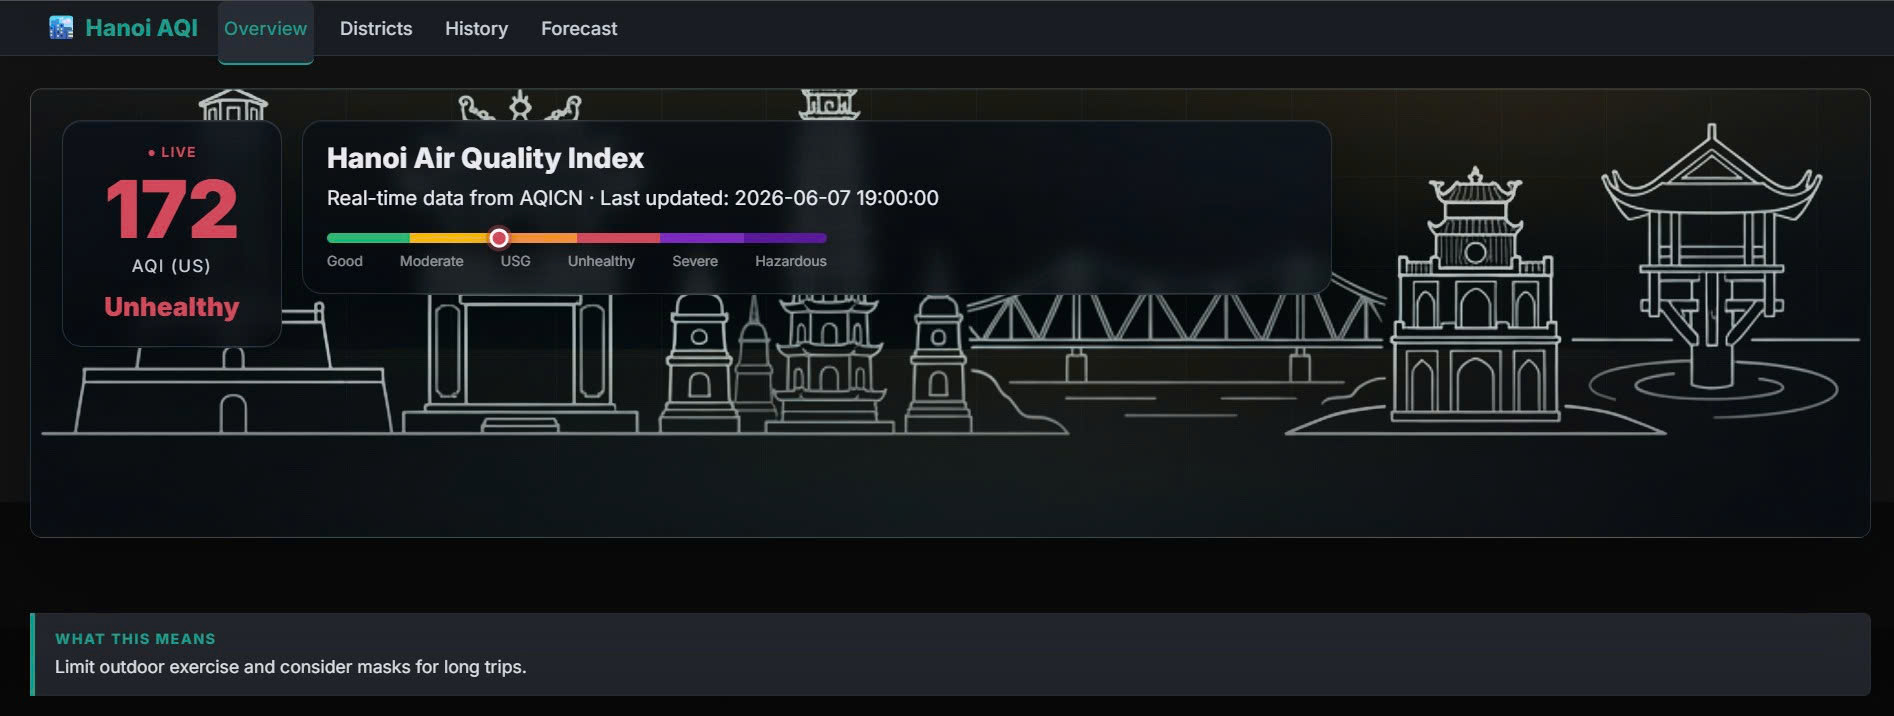
\includegraphics[width=\linewidth]{fig_overview_1.jpg}
\caption{Live hero AQI (172, ``Unhealthy'') on the six-band scale, AQICN timestamp, the Hanoi skyline
motif, and the plain-language ``what this means'' advisory.}
\end{subfigure}
\\[4pt]
\begin{subfigure}{0.7\textwidth}\centering
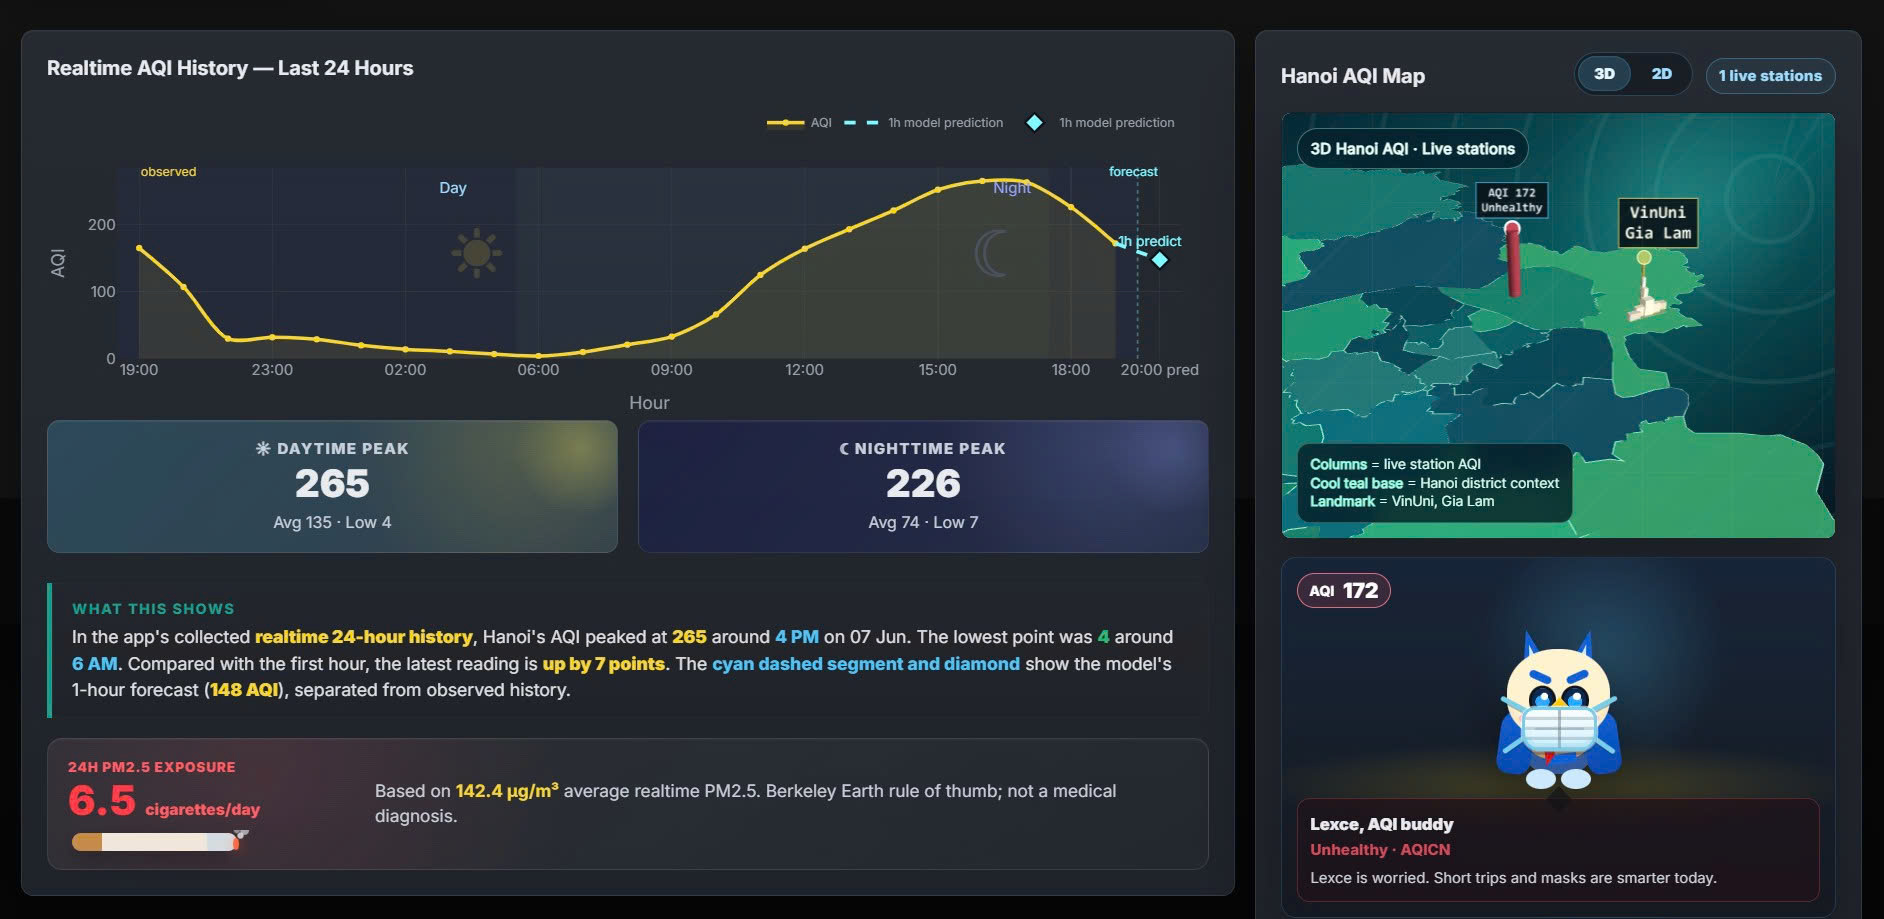
\includegraphics[width=\linewidth]{fig_overview_2.jpg}
\caption{The 24\,h realtime line with day/night shading and the cyan dashed 1\,h forecast; day/night peak
cards; PM2.5 ``cigarettes/day'' exposure; and the 3D Hanoi map with live station, VinUni landmark, and the
Lexce mascot.}
\end{subfigure}
\caption{Overview page: the present situation made glanceable, with observed vs.\ predicted clearly
distinguished.}
\label{fig:overview}
\end{figure}

\subsection{Districts --- spatial inequality, explorable}
\begin{designnotes}
\item[User goal:] find which districts are most polluted and how the ranking shifts by month/year.
\item[Encodings \& rationale:] a choropleth is the canonical value-per-region encoding; selected
districts are saturated while unselected ones dim to context. The ranking is a \emph{heatmap-table} ---
exact rank and value in a sortable table, with twelve month columns coloured by the AQI scale --- chosen
over a plain sorted bar chart because it preserves per-district \emph{seasonality} in the same view. A
multi-line monthly trend adds a dotted city-average baseline for reference, and a horizontal pollutant bar
breaks the selection into its six constituent pollutants.
\item[Interaction (the strongest coordinated-views story):] one district selection --- made by checkbox
or by a preset (\textit{Top~5}, \textit{Above avg}, \textit{PM2.5 hotspots}, \textit{Select all},
\textit{Clear}) --- simultaneously filters the map, ranking table, trend, and breakdown. Year/month
controls re-aggregate the map and ranking while the trend retains year context, so a filter never strands
the user without comparison. Figure~\ref{fig:districts} shows the linked layout.
\item[Key insight:] citywide averages hide real spatial disparities, and linked selection lets users
attribute high months to specific districts.
\item[Narrative link:] the \emph{space} axis of the story.
\end{designnotes}

\begin{figure}[H]
\centering
\begin{subfigure}{0.7\textwidth}\centering
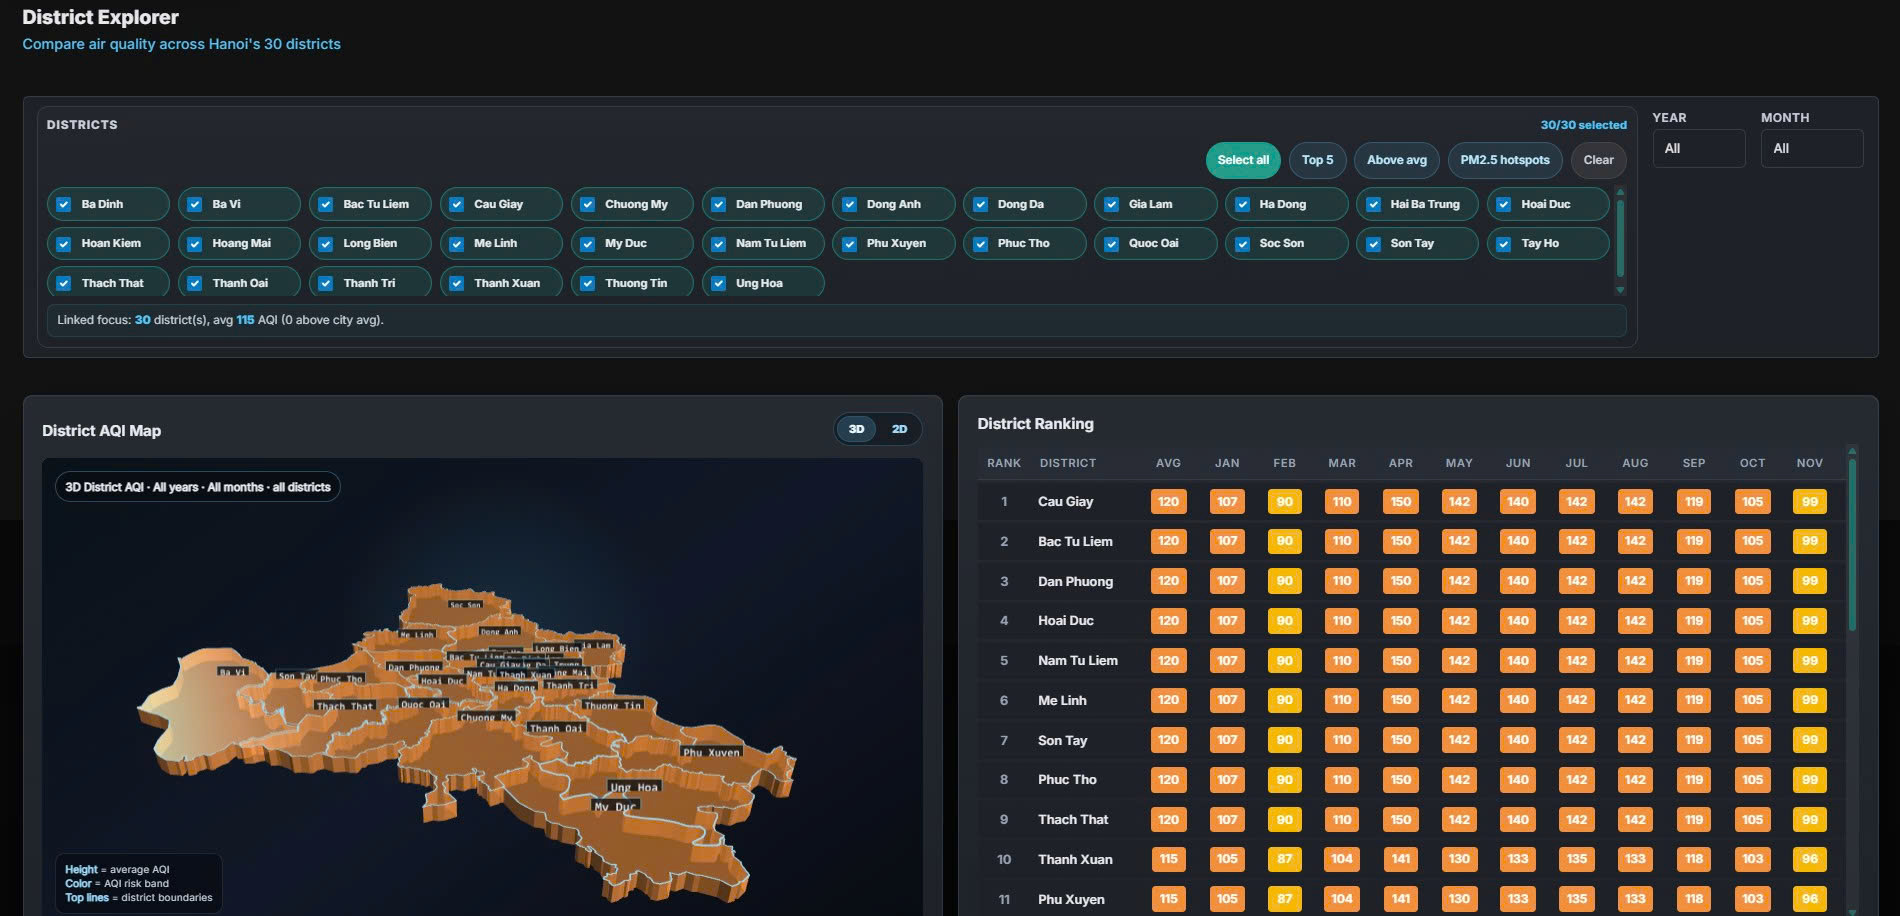
\includegraphics[width=\linewidth]{fig_districts_1.jpg}
\caption{District selector with presets (Top~5, Above avg, PM2.5 hotspots\ldots) and year/month controls;
the 3D extruded choropleth; and the ranking table with twelve AQI-coloured month columns.}
\end{subfigure}
\\[4pt]
\begin{subfigure}{0.7\textwidth}\centering
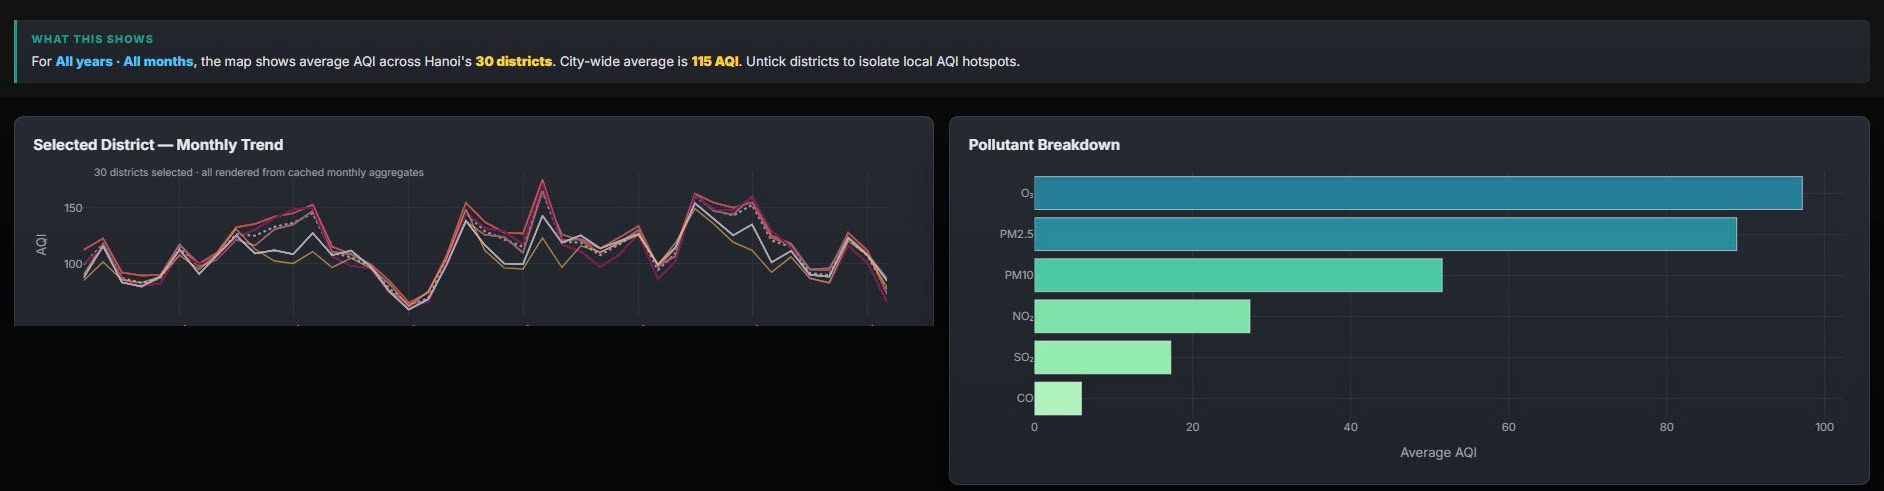
\includegraphics[width=\linewidth]{fig_districts_2.jpg}
\caption{The linked monthly trend (selected districts vs.\ a dotted city baseline) and the pollutant
breakdown bar --- both react to the same selection.}
\end{subfigure}
\caption{Coordinated multiple views on the Districts page: a single selection drives map, ranking, trend,
and pollutant breakdown together.}
\label{fig:districts}
\end{figure}

\subsection{History --- temporal rhythm and honest anomalies}
\begin{designnotes}
\item[User goal:] see daily, seasonal, and multi-year patterns and inspect unusual events.
\item[Encodings \& rationale:] a GitHub-style \emph{calendar heatmap} (day-of-week $\times$ week, AQI
colour) makes an entire year of daily values scannable at once and surfaces seasonal bands and bad-day
clusters far better than a long line chart. A multi-year \emph{seasonal overlay} plots the same selected
month across years (current year bold) to separate seasonal signal from year-to-year drift. A category
donut and a month$\times$year stacked-bar matrix give part-to-whole and small-multiple views of how the
mix of Good$\rightarrow$Hazardous days evolves.
\item[Interaction:] pollutant (AQI/PM2.5/PM10), year, and month selectors re-target the views, and a
\emph{``show anomaly markers''} toggle overlays flagged days (red ``$\times$'') \emph{only on request} (Figure~\ref{fig:history}).
This reveal-on-demand choice keeps production views clean while preserving the ability to audit
data-quality events --- analytical honesty without clutter.
\item[Key insight:] Hanoi air quality has strong temporal structure; clean visuals and on-demand
anomaly inspection can coexist.
\item[Narrative link:] the \emph{time} axis of the story.
\end{designnotes}

\begin{figure}[H]
\centering
\begin{subfigure}{0.7\textwidth}\centering
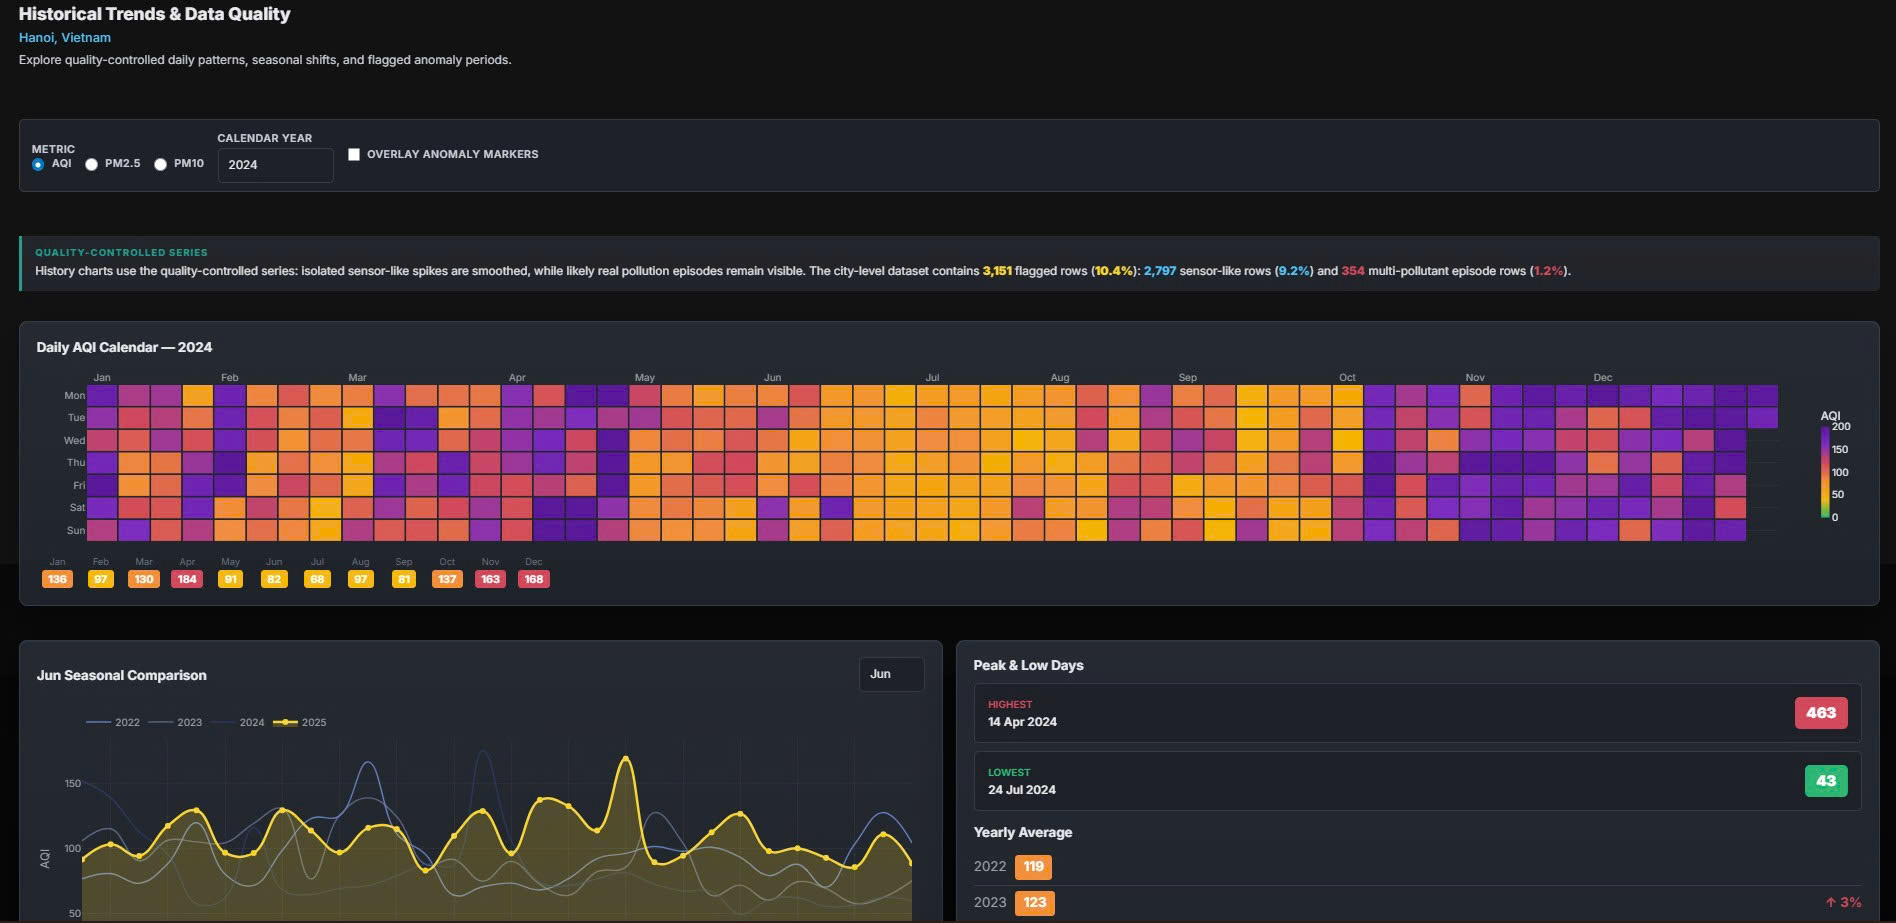
\includegraphics[width=\linewidth]{fig_history_1.jpg}
\caption{Metric/year controls and the anomaly-marker toggle; the quality-controlled-series note (flagged
vs.\ sensor-like vs.\ episode rows); the daily AQI calendar heatmap; and the multi-year seasonal overlay.}
\end{subfigure}
\\[4pt]
\begin{subfigure}{0.7\textwidth}\centering
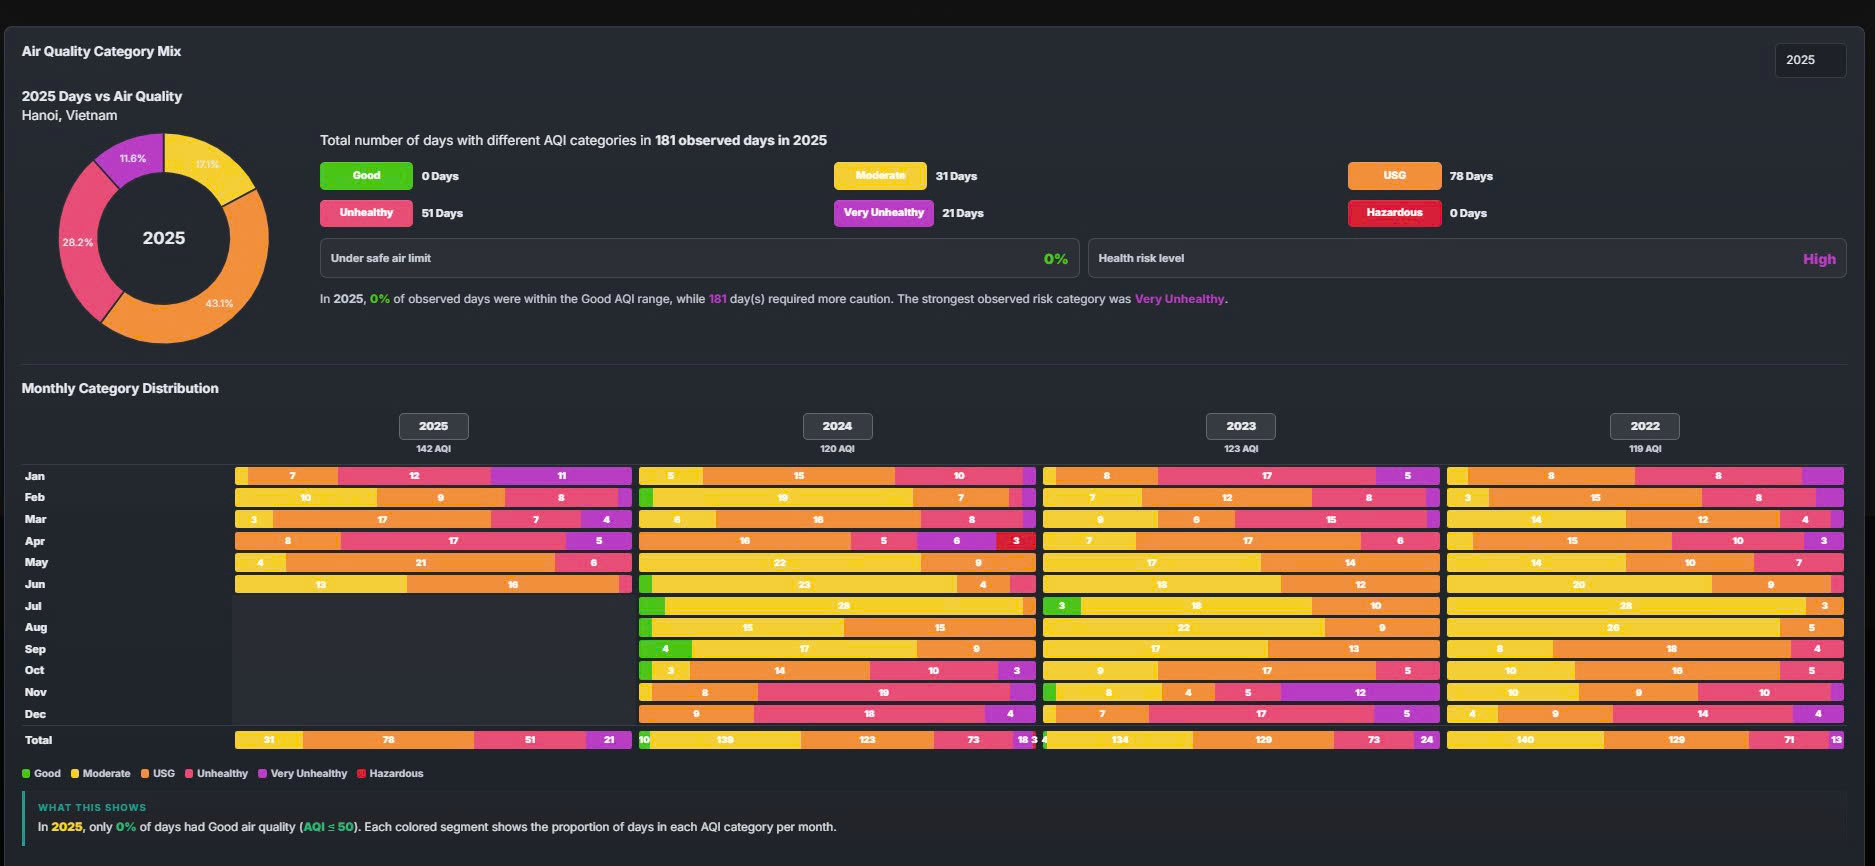
\includegraphics[width=\linewidth]{fig_history_2.jpg}
\caption{The air-quality category-mix donut and the month$\times$year stacked-bar matrix showing how the
Good$\rightarrow$Hazardous day mix shifts across seasons and years.}
\end{subfigure}
\caption{History page: daily, seasonal, and categorical views of the temporal record, with on-demand
data-quality inspection.}
\label{fig:history}
\end{figure}

\subsection{Forecast --- the future, made interpretable}
\begin{designnotes}
\item[User goal:] see short-term predicted risk and judge whether to trust it.
\item[Encodings \& rationale:] the forecast hero reuses the AQI scale and adds a \emph{source-tier chip}
(live input vs.\ historical fallback) so users see how grounded each prediction is. Rather than a single
number, three diagnostic views build trust: a \emph{Key-Drivers radar} (\texttt{Scatterpolar}, top-7
permutation-importance features) shows \emph{what} drives the forecast; a \emph{learning-space PCA}
scatter places the current case among historical backtest cases (coloured by error, target, or risk band)
to reveal high-error regions; and grouped \emph{model-vs-baseline} bars plus a backtest line give the
honest track record (Figure~\ref{fig:forecast}). The PCA view is explicitly labelled a projection of
engineered regression features, not a neural embedding.
\item[Interaction:] horizon (1/6/24~h) and target (AQI/PM2.5) radios reload the relevant cached model;
a PCA colour-mode toggle re-encodes without recomputation.
\item[Key insight:] a forecast is only useful if its drivers and error are visible --- so the page sells
interpretability, not just a value.
\item[Narrative link:] the \emph{future} axis, closing the space$\rightarrow$time$\rightarrow$future arc.
\end{designnotes}

\begin{figure}[H]
\centering
\begin{subfigure}{0.7\textwidth}\centering
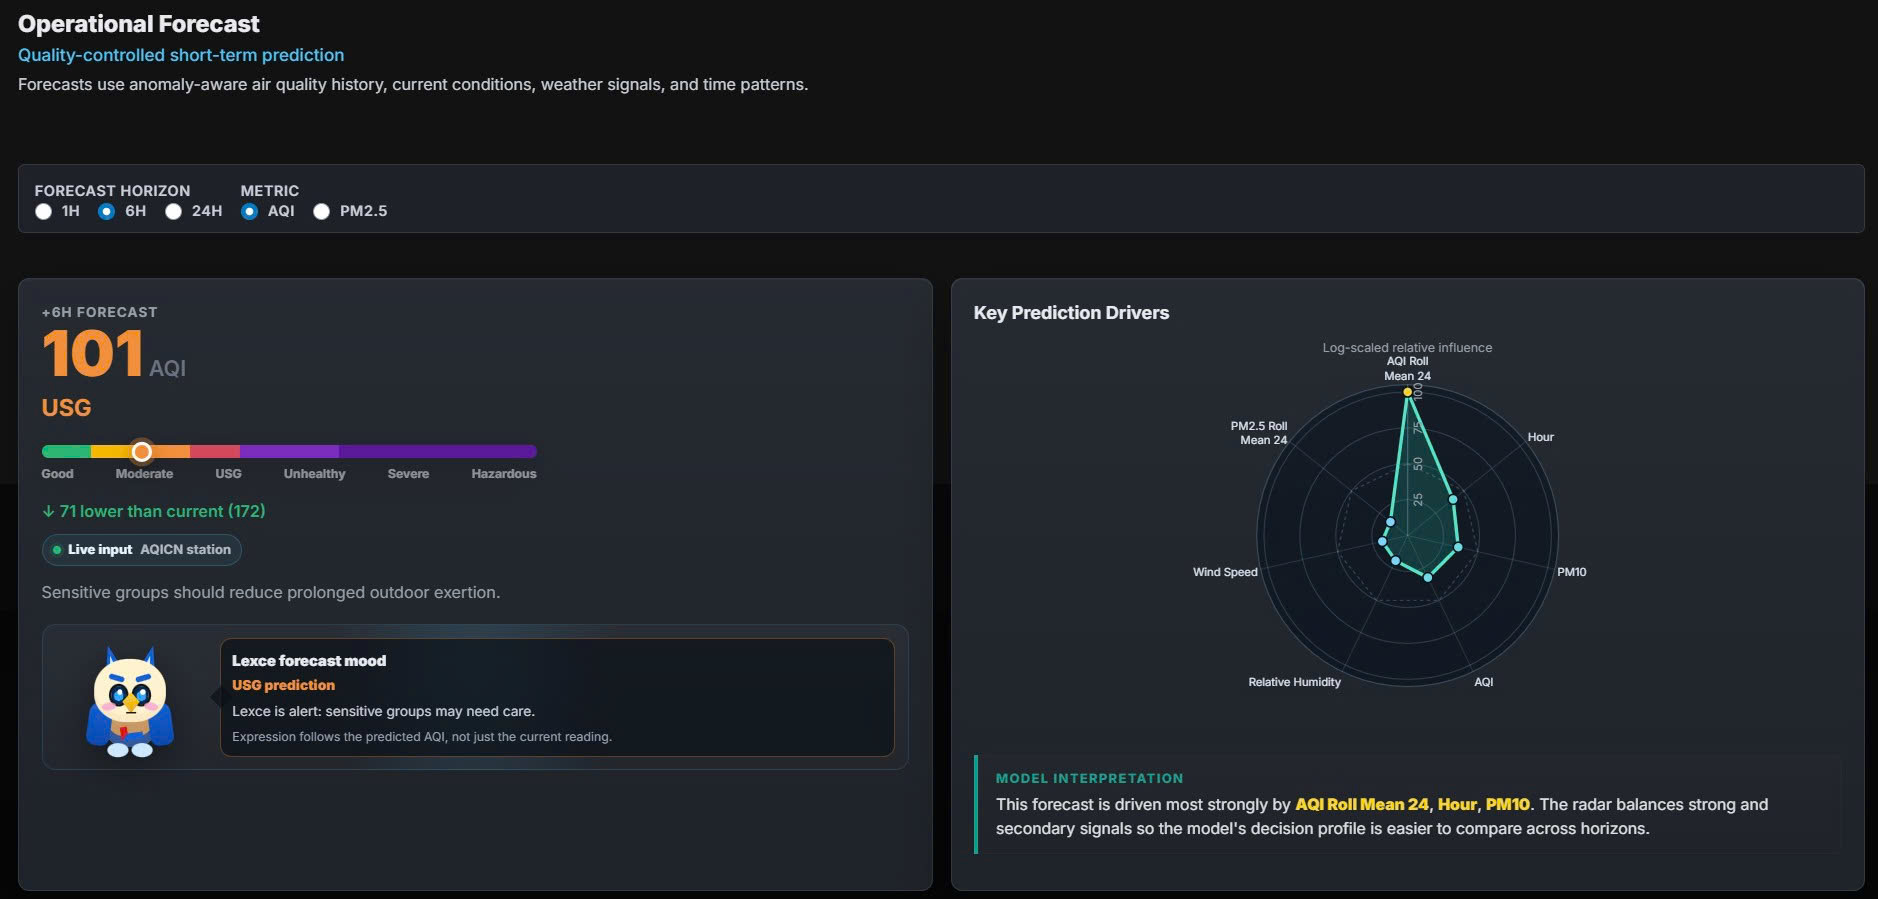
\includegraphics[width=\linewidth]{fig_forecast_1.jpg}
\caption{Horizon/target controls; the +6\,h forecast hero (101 AQI, USG) with the source-tier ``Live input''
chip and delta-from-current; the Lexce forecast mood; and the Key-Drivers radar of top features.}
\end{subfigure}
\\[4pt]
\begin{subfigure}{0.7\textwidth}\centering
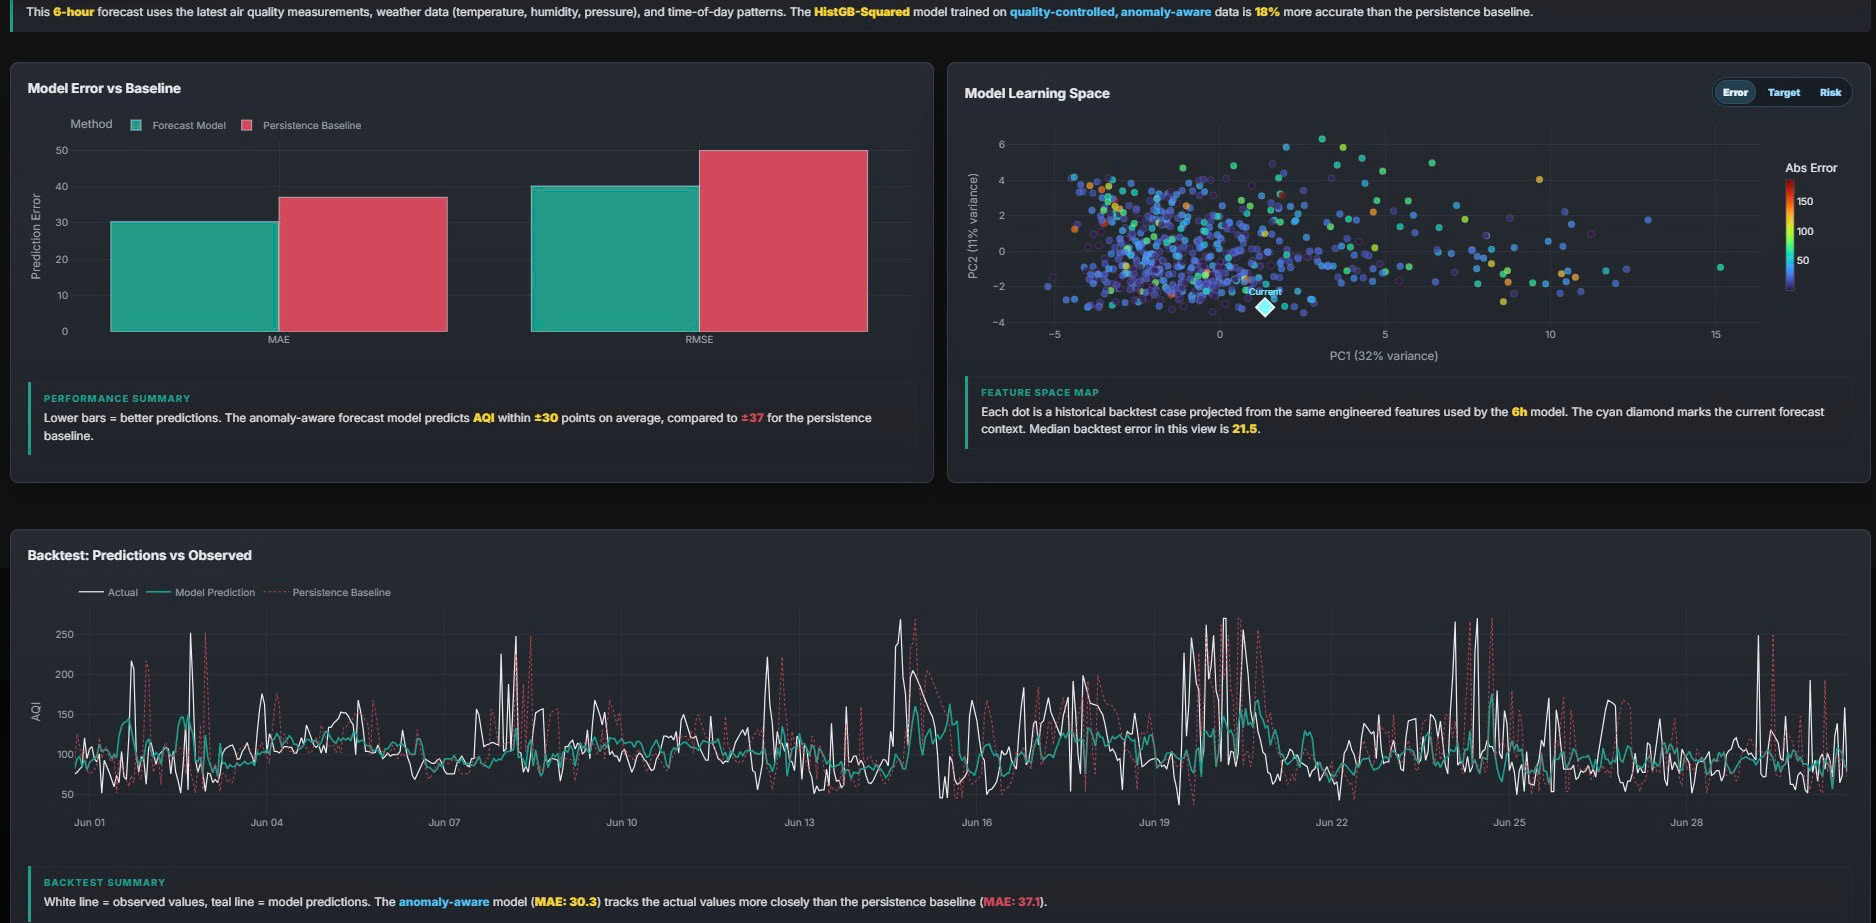
\includegraphics[width=\linewidth]{fig_forecast_2.jpg}
\caption{Model-vs-baseline error bars (MAE/RMSE), the PCA learning space (current case as a cyan diamond,
error/target/risk colour modes), and the backtest of model vs.\ persistence over a month.}
\end{subfigure}
\caption{Forecast page: prediction presented with interpretability devices (drivers, learning space,
backtest) rather than a single opaque number.}
\label{fig:forecast}
\end{figure}

\subsection{Coordinated views, storytelling, and accessibility}
The four pages are deliberately sequenced as one story: the Overview anchors the present, Districts opens
the spatial dimension, History the temporal, and Forecast the predictive. Within Districts, coordination
is literal --- a shared reactive selection links four charts so an observation in one is explained by the
others, following the coordinated-multiple-views principle. Throughout, every major view carries a small
\emph{``what this shows / what it means''} insight panel (an \texttt{aria-live} region) that updates with
the active filters, so interaction improves \emph{understanding}, not merely data subsetting. Accessibility
was treated as a design constraint, not an afterthought: 2D map alternatives to every 3D scene, keyboard
focus states, ARIA live regions, reduced-motion support, and high-contrast insight text.

%==================== 3. DATA & PREPROCESSING ====================
\section{Data and Preprocessing}
The application combines two historical Kaggle datasets, district boundaries, and live readings
(Table~\ref{tab:data}). The district source drives the spatial views; the city source drives the History
tab and all forecasting. Processed data is cached as compact Parquet to keep app startup fast, and forecast
models are trained offline and cached as Joblib artifacts so deployment never retrains during a demo.

\begin{table}[h]
\centering
\small
\begin{tabular}{@{}lllr@{}}
\toprule
Dataset & Source & Coverage & Rows \\
\midrule
District (30 districts) & Kaggle \texttt{hau100416/vietnamese-air-quality-dataset} & 2022-08-04 to 2026-02-01 & 920{,}160 hourly \\
City (Hanoi) & Kaggle \texttt{phungdinhdat/aqi-in-hanoi-2022-2025} & 2022-01-13 to 2025-06-30 & 30{,}341 hourly \\
Boundaries & geoBoundaries VNM ADM2 (HDX fallback) & static & 30 polygons \\
Realtime & AQICN/WAQI + Open-Meteo fallback & live ($\le 48$\,h fresh) & --- \\
\bottomrule
\end{tabular}
\caption{Data sources. City fields include AQI, PM2.5, PM10, CO, NO\textsubscript{2}, O\textsubscript{3},
SO\textsubscript{2}, temperature, humidity, pressure, precipitation, wind, clouds, and UV index.}
\label{tab:data}
\end{table}

\paragraph{Anomaly-aware cleaning that protects the visuals.}
Air-quality series mix genuine pollution episodes with sensor artifacts, and uncritically plotting either
extreme would mislead. Preprocessing therefore (i)~enforces physical validity ranges (e.g.\ AQI
$0$--$500$, humidity $0$--$100$, pressure $950$--$1050$), (ii)~computes a robust local outlier score from a
72~h rolling median and MAD ($\sigma = 1.4826\,\text{MAD}$), flagging a point only when its robust
$z>6$ \emph{and} it exceeds a per-pollutant minimum delta, and (iii)~separates \emph{sensor-like} isolated
spikes from \emph{extreme episodes} where two or more pollutants spike together. The cleaned series clips
and interpolates sensor-like/invalid values but \textbf{preserves real episodes}. This is what lets the
History tab show a stable default view while still exposing flagged days through the anomaly toggle.
District names from the boundary file are matched to the dataset's ASCII names (diacritic mapping) so the
choropleths align with the data.

%==================== 4. TECHNICAL IMPLEMENTATION ====================
\section{Technical Implementation and Architecture}
The dashboard is built with Python Shiny using a module-per-tab pattern: \texttt{app.py} composes a navbar
of four \texttt{@module} UI/server pairs (\texttt{mod\_overview}, \texttt{mod\_district},
\texttt{mod\_history}, \texttt{mod\_forecast}) and holds shared reactive state (current snapshot, station
cache, realtime history, and a cache of model artifacts). Visualizations are Plotly; the 3D maps are
deck.gl scenes embedded as HTML iframes. A core \texttt{src/} library separates concerns: \texttt{data.py}
(load/normalize Parquet/CSV), \texttt{anomaly.py} (quality flags), \texttt{model.py} (features, training,
prediction), \texttt{realtime\_api.py} (WAQI + Open-Meteo), and \texttt{utils.py} (shared AQI helpers).

\paragraph{Realtime architecture (Figure~\ref{fig:arch}).}
Because shinyapps.io processes sleep when idle, realtime collection runs \emph{outside} the app. A SLURM
job runs \texttt{collect\_realtime\_history.py} roughly every 10 minutes, records the nearest Hanoi
station's reading, trims to a 168~h window, and uploads \texttt{realtime\_history.csv} to the Hugging Face
dataset \texttt{MountainRiver/hanoi-aqi-realtime-history}. The deployed app reads that CSV as its
lightweight history source, so the Overview page shows fresh data even when no session was previously open.
When AQICN is unavailable or incomplete, the app falls back to Open-Meteo or cleaned historical context,
and the forecast UI makes this explicit with source-tier chips. Reproducibility is supported by a pinned
\texttt{requirements.txt} and unit tests under \texttt{dashboard/tests/}.

\begin{figure}[H]
\centering
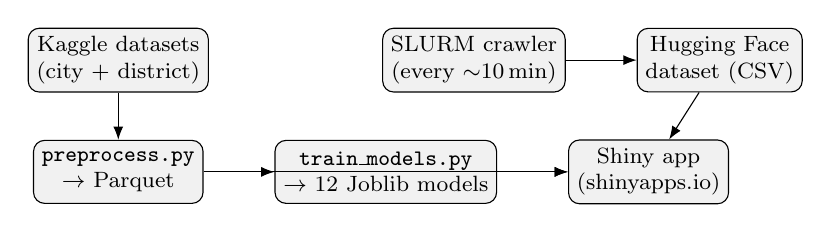
\begin{tikzpicture}[
    node distance=6mm and 9mm, font=\footnotesize,
    box/.style={draw, rounded corners, align=center, minimum height=8mm, inner sep=3pt, fill=Gainsboro!40},
    >=Latex]
\node[box] (kaggle) {Kaggle datasets\\(city + district)};
\node[box, below=of kaggle] (pre) {\texttt{preprocess.py}\\$\rightarrow$ Parquet};
\node[box, right=of pre] (train) {\texttt{train\_models.py}\\$\rightarrow$ 12 Joblib models};
\node[box, right=22mm of kaggle] (slurm) {SLURM crawler\\(every $\sim$10\,min)};
\node[box, right=of slurm] (hf) {Hugging Face\\dataset (CSV)};
\node[box, right=of train] (app) {Shiny app\\(shinyapps.io)};
\draw[->] (kaggle) -- (pre);
\draw[->] (pre) -- (train);
\draw[->] (slurm) -- (hf);
\draw[->] (hf) -- (app);
\draw[->] (train) -- (app);
\draw[->] (pre.east) -- ++(1.2,0) |- (app.west);
\end{tikzpicture}
\caption{Offline preprocessing/training plus an out-of-app SLURM realtime crawler feeding a Hugging Face
dataset that the deployed Shiny app reads back --- keeping the demo fresh and reproducible.}
\label{fig:arch}
\end{figure}

%==================== 5. FORECASTING AS COMPLEMENT ====================
\section{Forecasting as a Visual-Analytic Complement}
Forecasting is included to extend the visual workflow into the near future, not to replace it. Models
predict two targets (AQI, PM2.5) at three horizons (1/6/24~h) using current pollutants, weather, time
features (hour, day-of-week, month, weekend), lag features (1/6/24~h), and rolling mean/max windows
(3/6/24~h). The estimator is scikit-learn \texttt{HistGradientBoostingRegressor}, selected among three
candidate configurations by lowest error on a \emph{chronological} 80/20 split (no shuffling, to avoid
look-ahead leakage); the baseline is a persistence forecast. Table~\ref{tab:model} reports the cleaned-series
artifacts deployed in the app --- \textbf{these values were read directly from the trained
\texttt{.joblib} files}, not from documentation.

\begin{table}[h]
\centering
\small
\begin{tabular}{@{}llrrr@{}}
\toprule
Target / horizon & Selected model & Model MAE & Baseline MAE & Improvement \\
\midrule
AQI 1h    & HistGB-Absolute & 18.80 & 19.15 & $+1.8\%$ \\
AQI 6h    & HistGB-Squared  & 30.33 & 37.09 & $+18.2\%$ \\
AQI 24h   & HistGB-Absolute & 35.37 & 44.43 & $+20.4\%$ \\
PM2.5 1h  & HistGB-Absolute & 11.89 & 11.73 & $-1.4\%$ \\
PM2.5 6h  & HistGB-Absolute & 20.82 & 25.64 & $+18.8\%$ \\
PM2.5 24h & HistGB-Absolute & 24.59 & 29.94 & $+17.9\%$ \\
\bottomrule
\end{tabular}
\caption{Verified cleaned-series model performance (mean absolute error vs.\ persistence baseline). Gains
grow with horizon, where persistence weakens; the $-1.4\%$ at PM2.5 1h is an honest limitation --- for very
short-term PM2.5 the baseline is already strong.}
\label{tab:model}
\end{table}

The dashboard shows baseline error alongside model error precisely so this nuance is visible rather than
hidden behind a single forecast number. The radar, PCA learning-space, and backtest views (Section~2.4)
exist to make the model interpretable inside the visualization, which is the project's stance on
forecasting: a transparent complement to exploration.

%==================== 6. FINDINGS, LIMITATIONS, FUTURE WORK ====================
\section{Findings, Limitations, and Future Work}
\textbf{Findings.} The coordinated design surfaces patterns a single AQI number cannot: clear diurnal and
seasonal structure (Overview day/night summaries, History seasonal overlay and calendar), spatial
inequality that linked district selection can attribute to specific districts and months, and a forecast
layer that beats persistence at 6 and 24~h while honestly under-performing at PM2.5 1h. The anomaly-aware
design lets clean production charts and on-demand data-quality inspection coexist.

\textbf{Limitations.} Realtime station coverage can be sparse or stale, and the crawler currently stores
only AQI, PM2.5, PM10, coordinates, source, and timestamps --- not every weather/secondary-pollutant
feature used in training --- so live forecasts use fallback context for missing features; this is shown in
the UI but should not be overstated as a fully realtime feature pipeline. Forecasting is city-level rather
than district-specific, and the 3D maps are visual encodings of magnitude, not physical terrain or
building heights.

\textbf{Future work.} Store richer realtime weather/pollutant features, add uncertainty bands to forecasts,
train district-specific models where data density allows, and conduct formal accessibility user testing;
a longer-term version could add alerts and location-specific, uncertainty-aware exposure recommendations.

%==================== REFERENCES ====================
\begin{thebibliography}{9}
\small
\bibitem{hau} Kaggle dataset, \texttt{hau100416/vietnamese-air-quality-dataset}.
\bibitem{phung} Kaggle dataset, \texttt{phungdinhdat/aqi-in-hanoi-2022-2025}.
\bibitem{aqicn} AQICN / WAQI realtime air-quality station data. \url{https://aqicn.org}
\bibitem{openmeteo} Open-Meteo air-quality and weather APIs. \url{https://open-meteo.com}
\bibitem{geo} geoBoundaries (VNM ADM2) administrative boundaries. \url{https://www.geoboundaries.org}
\bibitem{stack} Python Shiny, Plotly, deck.gl, pandas, scikit-learn, Hugging Face Hub.
\end{thebibliography}

\end{document}
